\appendix

\section{The \textit{Asix Sigma2} logic analyser}
\label{ap:la}

The Asix Sigma2 logic analyser is like:\\ 
\begin{center}
    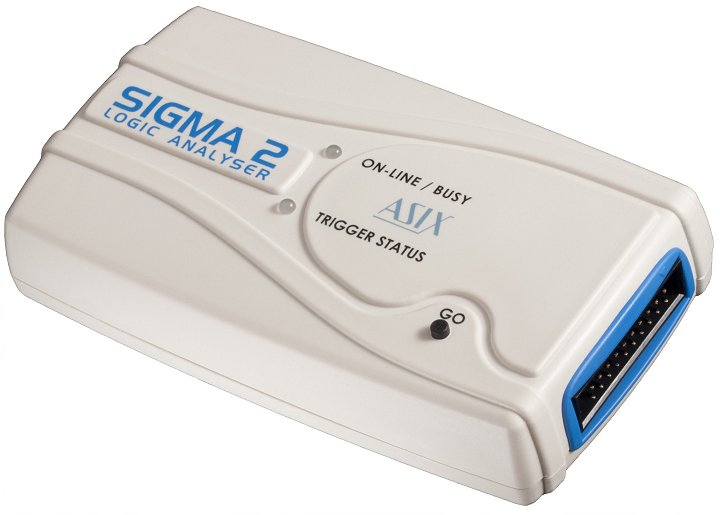
\includegraphics[width=4cm]{sigma2_720x515.jpg}
\end{center}

\subsection{Electrical connections to the Explorer 16 board}
    Connect the analyser to the extension board with the numbered ribbon cable following this scheme:
    \begin{center}
        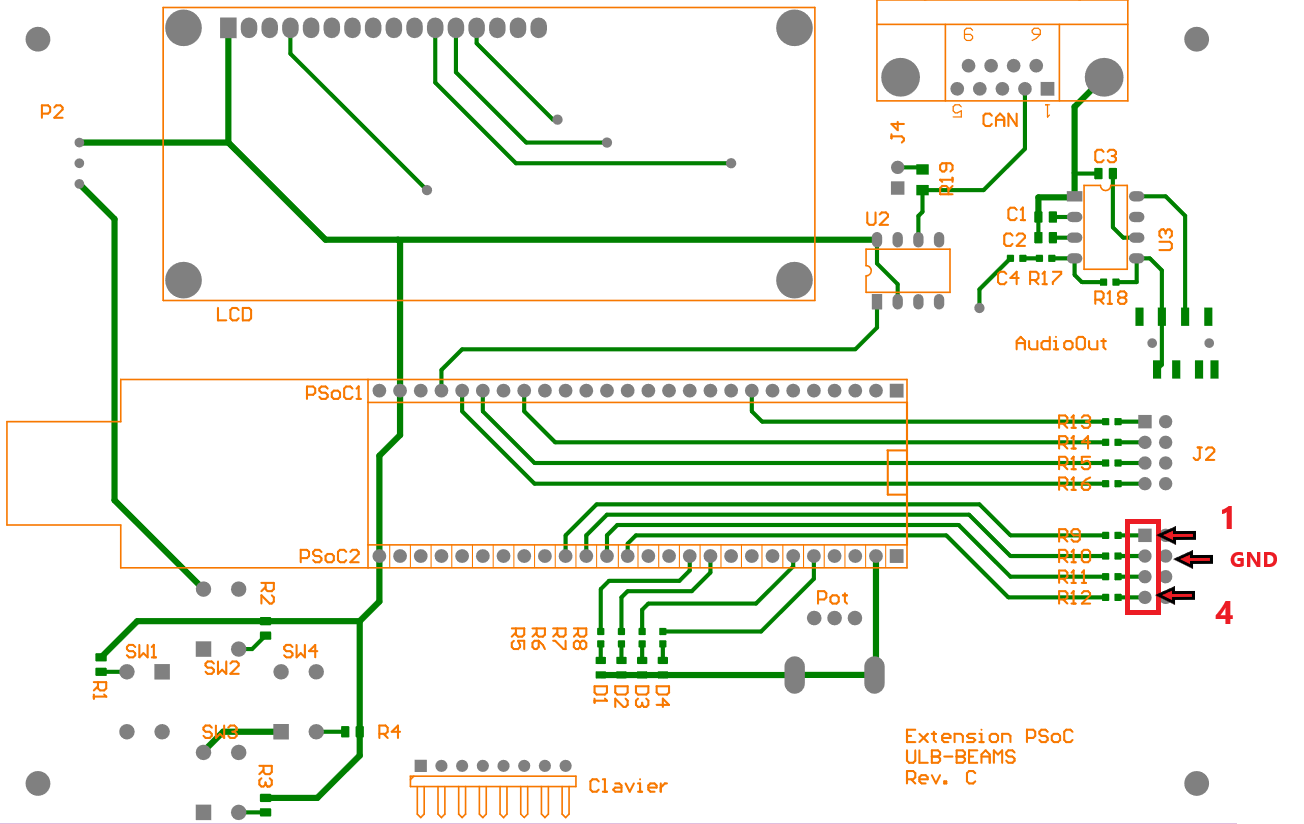
\includegraphics[width=0.7\textwidth]{analyserConnection.png}
    \end{center}

\subsection{Software on the computer}
    The software interface of the logic analyser looks like:
    \begin{center}
    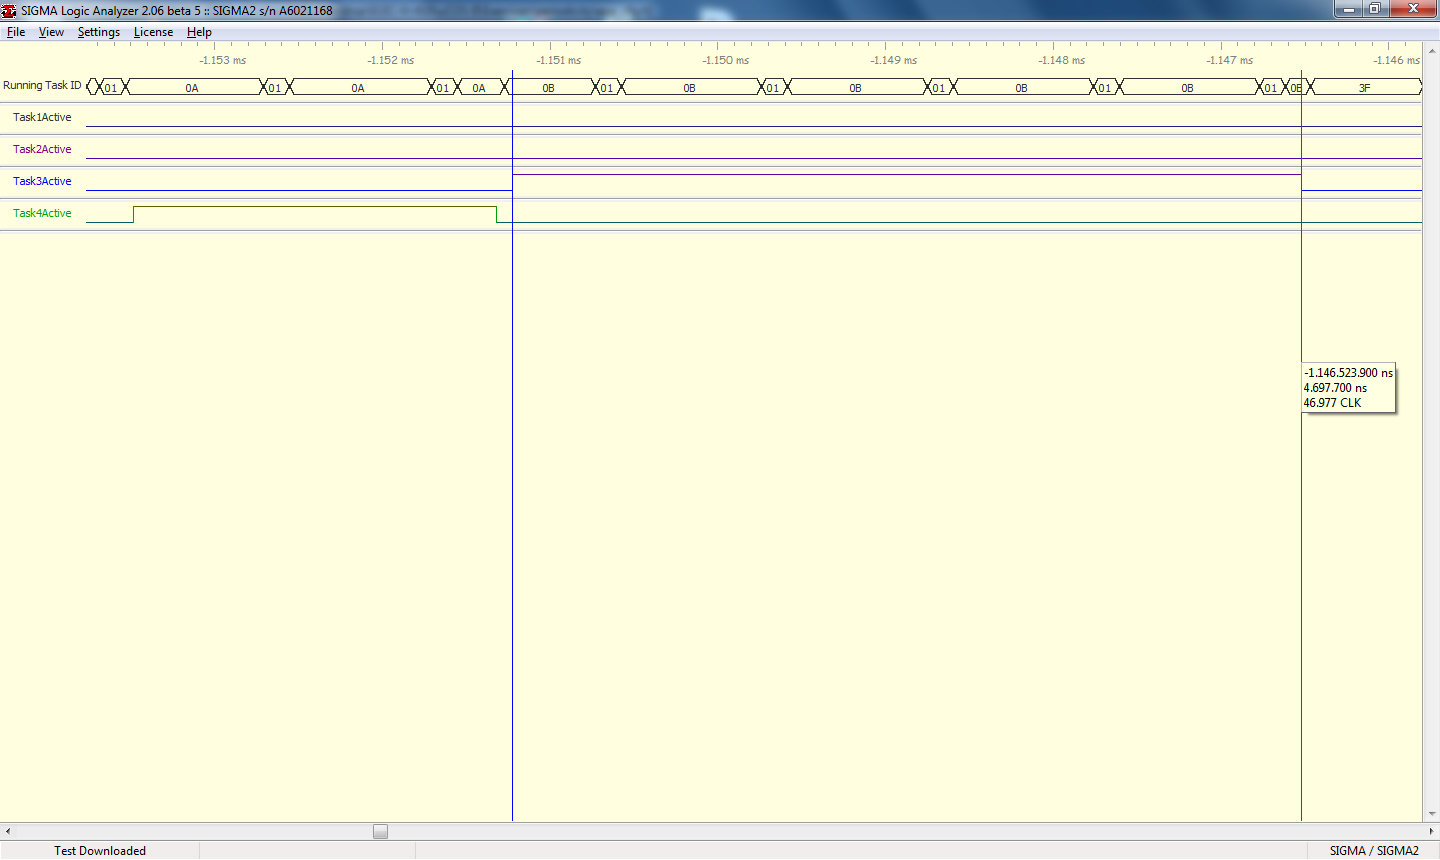
\includegraphics[width=13cm,trim= 0 100mm 0 0,clip]{Print_Screen_Logic_Analyzer.png}
    \end{center}

\subsection{Basic measurements}
    The red line on the screen is a cursor showing the time and values of signals in the main window. To place a marker (blue line), press space. If you move your cursor, the difference between the marker and the cursor will show in a tooltip.

    The first acquisition must be launched by software. Following acquisitions can be done using the ``go" button of the analyser.
